%@ Subject: Elementary Probability
\addpoints
\question[20] El $5\%$  de las unidades producidas en una fábrica se encuentran defectuosas cuando el proceso de fabricación se encuentra bajo control. Si el proceso se encuentra fuera de control, se produce un $30\%$ de unidades defectuosas. Se sabe, además, que la probabilidad de que un proceso se encuentre bajo control es de $0,92$. 
\noaddpoints
\begin{parts}
\part[3] Defina sucesos e identifique probabilidades.
\part[7] ¿Cuál es la probabilidad de que una unidad producida sea defectuosa?.
\part[10] Si se escoge aleatoriamente una unidad y se encuentra que es defectuosa, ¿Cuál es la probabilidad de que el proceso haya estado bajo control?

\end{parts}

\begin{solution}
\begin{enumerate}[a)]
\item Sintetizando la información por enunciado, las probabilidades respectivas están dadas por: 
\begin{center}
% Set the overall layout of the tree
\tikzstyle{level 1}=[level distance=3.5cm, sibling distance=3.5cm]
\tikzstyle{level 2}=[level distance=3.5cm, sibling distance=2cm]

% Define styles for bags and leafs
\tikzstyle{bag} = [text width=4em, text centered]
\tikzstyle{end} = [circle, minimum width=3pt,fill, inner sep=0pt]

% The sloped option gives rotated edge labels. Personally
% I find sloped labels a bit difficult to read. Remove the sloped options
% to get horizontal labels. 
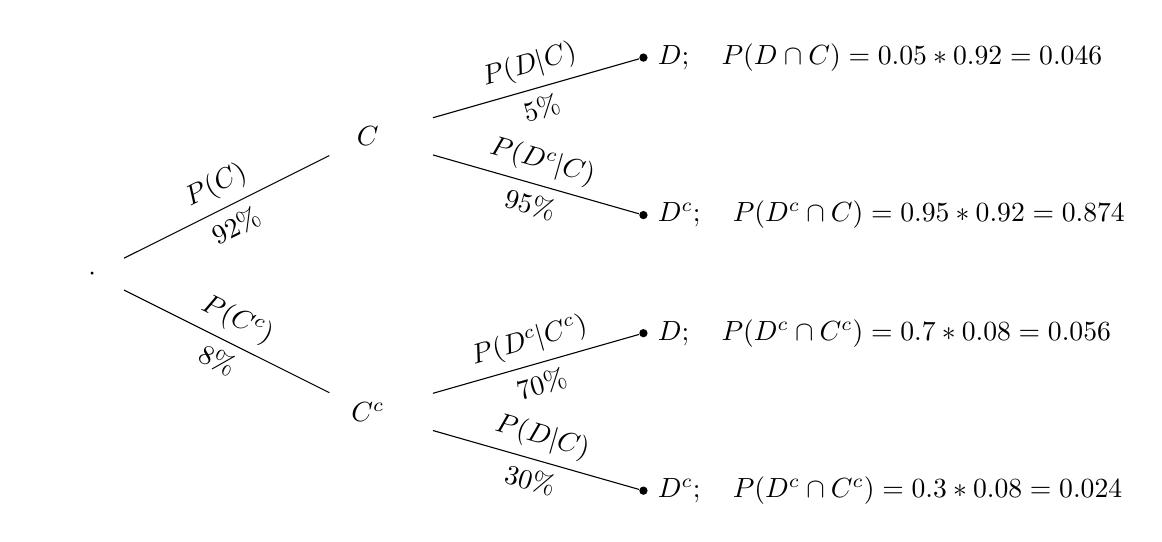
\begin{tikzpicture}[grow=right, sloped]
\node[bag] {$\cdot$}
    child {
        node[bag] {$C^c$}        
            child {
                node[end, label=right:
                    {$D^c; \hspace{10pt}\mathbb{P}(D^c\cap C^c)=0.3*0.08=0.024$}] {}
                edge from parent
                node[above] {$\mathbb{P}(D|C)$}
                node[below]  {$30\%$}
            }
            child {
                node[end, label=right:
                    {$D; \hspace{10pt}\mathbb{P}(D^c\cap C^c)=0.7*0.08=0.056$}] {}
                edge from parent
                node[above] {$\mathbb{P}(D^c|C^c)$}
                node[below]  {$70\%$}
            }
            edge from parent 
            node[above] {$\mathbb{P}(C^c)$}
            node[below]  {$8\%$}
    }
    child {
        node[bag] {$C$}        
        child {
                node[end, label=right:
                    {$D^c; \hspace{10pt}\mathbb{P}(D^c\cap C)=0.95*0.92=0.874$}] {}
                edge from parent
                node[above] {$\mathbb{P}(D^c|C)$}
                node[below]  {$95\%$}
            }
            child {
                node[end, label=right:
                    {$D; \hspace{10pt}\mathbb{P}(D\cap C)=0.05*0.92=0.046$}] {}
                edge from parent
                node[above] {$\mathbb{P}(D|C)$}
                node[below]  {$5\%$}
            }
        edge from parent         
            node[above] {$\mathbb{P}(C)$}
            node[below]  {$92\%$}
    };
\end{tikzpicture}
\end{center}
En donde,\\
\begin{center}
$C:\{$ El proceso de fabricación se encuentra bajo control $\}$\\
$D:\{$ La(s) unidad(es) producida(s) es(son) defectuosa(s) $\}$
\end{center}
Y además, definiendo los sucesos complemento de forma análoga se tiene lo pedido.
\newpage
\item \begin{align*}
\mathbb{P}(D)&=\mathbb{P}(C)*\mathbb{P}(D|C)+\mathbb{P}(C^c)*\mathbb{P}(D|C^c)\\
&=0.92*0.05+0.08*0.3\\
&=0.07 
\end{align*}
\item De la pregunta anterior, $\mathbb{P}(D)=0.07$ y $\mathbb{P}(D|C)=\dfrac{\mathbb{P}(D\cap C)}{\mathbb{P}(C)}=0.05$ , en donde $\mathbb{P}(C)=0.92$, luego $\mathbb{P}(D\cap C)=0.05*0.92=0.046 \Rightarrow \mathbb{P}(C|D)=\dfrac{0.046}{0.07}\approx 0.6571$ 
\end{enumerate}
\end{solution}